%%==================================================================%%
%% Author : Tejedo Gonz�lez, Daniel                                 %%
%%          S�nchez Barreiro, Pablo                                 %%
%% Version: 1.0, 10/12/2012                                         %%                   %%                                                                  %%
%% Memoria del Proyecto Fin de Carrera                              %%
%% semantica, archivo ra�z                                       %%
%%==================================================================%%

\chapterheader{Sem�ntica del lenguaje}{Implementaci�n de la Sem�ntica, Integraci�n y Despliegue}
\label{chap:semantica}

Este cap�tulo describe la �ltima parte del proceso de desarrollo de nuestro lenguaje: la creaci�n de una sem�ntica que permita la evaluaci�n de las expresiones. Tras las implementaci�n de dicha sem�ntica, se procedi� a la integraci�n del editor creado en el entorno de desarrollo Eclipse, y a su posterior empaquetamiento y despliegue.

\chaptertoc

\section{Introducci�n}
\label{sec:sem:intro}

\todo{Escribe una intro}

\section{Implementaci�n de la sem�ntica del lenguaje}
\label{sec:sem:sem}
%%==================================================================%%
%% Author : Tejedo Gonz�lez, Daniel                                 %%
%%          S�nchez Barreiro, Pablo                                 %%
%% Version: 1.0, 10/12/2012                                         %%                   
%% Version: 2.0, 11/03/2013                                         %%                   
%%                                                                  %%
%% Memoria del Proyecto Fin de Carrera                              %%
%% semantica, semantica                                             %%
%%==================================================================%%

La implementaci�n la sem�ntica del lenguaje es el �ltimo paso que restaba para dar por concluido el desarrollo de nuestro lenguaje. La sem�ntica del lenguaje hab�a sido especificada  informalmente por el profesor Pablo S�nchez de acuerdo a la estrategia descrita en la Secci�n~\ref{sec:meta:requisitos}.

El primer paso para poder evaluar las restricciones era cargar un fichero de configuraci�n para el �rbol de caracter�sticas sobre el cual definir las restricciones. Dicho de otra forma, era necesario cargar una selecci�n de caracter�sticas del �rbol de caracter�sticas original, con objeto de comprobar que dicha selecci�n satisfac�a las restricciones especificadas. 

El proceso de evaluaci�n por tanto, analiza si cada restricci�n se eval�a a verdadero o falso. Si una restricci�n se eval�a a falso, el resultado de la evaluaci�n ser� negativo. Cada restricci�n evaluada a falso se guarda en una lista que se utilizar� al final del proceso de validaci�n para construir un informe de incidencias que se mostrar� al usuario. 

La sem�ntica del lenguaje se ha implementado en Java, a�adiendo operaciones con la l�gica de evaluaci�n a cada metaclase del metamodelo de nuestro lenguaje (ver Secci�n~\ref{figmetameta}. Concretamente, a�adimos un m�todo \emph{evaluate} a las diferentes metaclases involucradas en restricciones, y aprovechamos la estructura arb�rea de las restricciones para evaluarlas de forma recursiva. Por ejemplo, el m�todo evaluate de la clase \emph{Plus} simplemente retornar� el valor num�rico de la suma del valor de su primer operando y del valor su segundo operando. Para ello es necesario evaluar primero los operandos, los cuales vez pueden ser a su vez operaciones num�ricas. Cada m�todo \emph{evaluate} recibe como par�metro la configuraci�n (selecci�n de caracter�sticas) sobre la que hay que realizar la evaluaci�n; y la caracter�stica que sirve como contexto para la evaluaci�n de dicha expresi�n.

Evaluar un n�mero simplemente consiste en retornar su valor. Evaluar una caracter�stica simple consiste en comprobar si est� seleccionada. Si es as� se eval�a a verdadero, sino se eval�a a falso. Evaluar una caracter�stica m�ltiple consiste en comprobar cu�ntas veces ha sido clonada. Si una caracter�stica, simple o m�ltiple, se tuviese que evaluar en un contexto, s�lo se considerar�a el sub�rbol cuya ra�z es la caracter�stica que act�a de contexto.

En general, la implementaci�n del m�todo \emph{evaluate} para la mayor�a de las operaciones es trivial y no conlleva m�s de un par de l�neas de c�digo (como el caso de la suma anteriormente comentado). No obstante, algunas operaciones son algo m�s complicadas y requieren algo m�s de reflexi�n, como, por ejemplo, las operaciones con contexto. Como se ha comentado con anterioridad, las operaciones con contexto se restringen a un sub�rbol del �rbol de configuraci�n. Por tanto, para buscar una caracter�stica simple o contar el n�mero de instancias de una caracter�stica m�ltiple, debemos buscar s�lo desde la ra�z del correspondiente sub�rbol hacia abajo. 

Tras implementar la sem�ntica del lenguaje, realizamos la interfaz para poder ejecutarla debidamente.




\section{Pruebas}
\label{sec:sem:pruebas}

\todo{Escribir algo sobre las pruebas de la sem�ntica}

\section{Integraci�n con Eclipse}
\label{sec:sem:int}
%%==================================================================%%
%% Author : Tejedo Gonz�lez, Daniel                                 %%
%%          S�nchez Barreiro, Pablo                                 %%
%% Version: 1.0, 10/12/2012                                         %%                   
%% Version: 2.0, 11/03/2013                                         %%                   
%%                                                                  %%
%% Memoria del Proyecto Fin de Carrera                              %%
%% semantica, interfaz                                              %%
%%==================================================================%%

Una vez implementada y probada la sem�ntica del lenguaje, lo �nico que nos quedaba era integrar el editor generado y su sem�ntica en en entorno Eclipse y en la herramienta Hydra. La Figura~\ref{figeditor} muestra la interfaz del editor en funcionamiento. Las caracter�sticas del editor creado por defecto por EMFText no eran suficientes para satisfacer todos los requisitos de nuestra aplicaci�n. El editor generado permit�a procesar ficheros de restricciones, pero no evaluarlos sobre configuraciones concretas. Para poder realizar esta operaci�n de validaci�n, a�adimos a Eclipse un bot�n denominado \emph{Validate}. Dicho bot�n, al ser pulsado, permite cargar una configuraci�n del modelo de caracter�sticas al cual se refiere nuestro fichero de restricciones. Una vez cargado, el manejador del bot�n inicia el proceso de validaci�n descrito en la secci�n anterior. A la conclusi�n del proceso de validaci�n, se recoge el informe generado por el proceso de validaci�n y se muestra al usuario.

\begin{figure}[!tb]
    \includegraphics[scale=0.135]{semantica/editor.eps}
    \caption{Interfaz gr�fica del editor para el lenguaje HCL. El c�rculo rojo muestra el bot�n a�adido para la validaci�n de las restricciones.}
    \label{figeditor}
\end{figure}

Tras la implementaci�n de este bot�n, se comprob� su correcto funcionamiento mediante diversas pruebas, proporcion�ndole, por ejemplo, ficheros de configuraci�n tanto v�lidos e inv�lidos. Tras esto, se concluy� la implementaci�n del editor para el lenguaje \emph{Hydra Constraint Language}, pudiendo proceder a su empaquetado y distribuci�n.

%%=============================================================================%%
%% NOTA(Pablo): Esta figura sobra. Se�ala el bot�n sobre la otra imagen        %%  
%%=============================================================================%%
%%
%% \begin{figure}[t]
%%      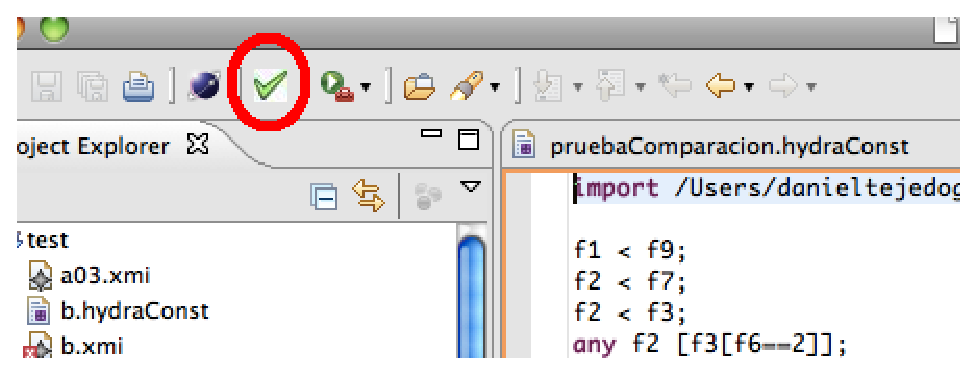
\includegraphics[scale=0.74]{semantica/boton.eps}
%%      \caption{Bot�n que ejecutar� la validaci�n de las restricciones}
%%      \label{figboton}
%% \end{figure}
%% 
%%=============================================================================%%



\section{Empaquetamiento y Despliegue}
\label{sec:sem:despliegue}
% %%==================================================================%%
%% Author : Tejedo Gonz�lez, Daniel                                 %%
%%          S�nchez Barreiro, Pablo                                 %%
%% Version: 1.0, 10/12/2012                                         %%                   
%% Version: 2.0, 11/03/2013                                         %%                   
%%                                                                  %%
%% Memoria del Proyecto Fin de Carrera                              %%
%% semantica, despliegue                                              %%
%%==================================================================%%

Una vez que se ha implementado la aplicaci�n completamente, el �ltimo paso para finalizar este proyecto es exportarla para que pueda ser utilizada en otros computadores.

Para llevar a cabo esta tarea se ha optado por la creaci�n de un \emph{update site}, que permite instalar la aplicaci�n desde la opci�n \emph{Install New Software} del propio men� de Eclipse. Consideramos que esta era la opci�n m�s c�moda de distribuir nuestra aplicaci�n. El archivo \emph{updateSite.zip} del CD adjunto contiene los ficheros necesarios para llevar a cabo la instalaci�n de nuestro editor.

Adem�s, hemos creado un peque�o manual de usuario que explica de manera r�pida y con muchas im�genes como empezar a utilizar nuestra aplicaci�n. Tambi�n hemos grabado un videotutorial que muestra la aplicaci�n en funcionamiento. Tanto el manual como el v�deo est�n disponibles en el CD adjunto, bajo el nombre de \emph{manual.pdf} y \emph{video.mp4}.

\todo{Escribir algosobre el empaquetamiento y despliegue}

\section{Sumario}
\label{sec:sem:sumario}
% %%==================================================================%%
%% Author : Tejedo Gonz�lez, Daniel                                 %%
%%          S�nchez Barreiro, Pablo                                 %%
%% Version: 1.0, 25/11/2012                                         %%                   
%%                                                                  %%
%% Memoria del Proyecto Fin de Carrera                              %%
%% Sintaxis abstracta, sumario                          %%
%%==================================================================%%

Durante el presente cap�tulo se ha descrito el proceso de definici�n de la sintaxis abstracta de nuestro lenguaje. Este proceso abarca subtareas como la captura de requisitos del lenguaje, la creaci�n de un metamodelo que permita la creaci�n de sintaxis concretas apropiadas, la validaci�n de restricciones externas a ese metamodelo, y las pruebas que corroboren que todos los elementos creados funcionan correctamente. En el siguiente cap�tulo profundizaremos acerca del dise�o de la gram�tica para nuestro lenguaje, as� como de las herramientas utilizadas para implementar esa gram�tica.

\todo{Escribir un sumario}

